\documentclass[10pt]{report}

\usepackage{amssymb}
\usepackage{amsmath}
\usepackage[numbered,autolinebreaks]{mcode}
\usepackage{graphicx}
\usepackage{verbatim}

\newcommand*{\gam}{$\gamma \text{ }$}
\newcommand*{\gami}{$\gamma_{i} \text{ }$}
\newcommand*{\pdivq}{$\frac{p}{q} \text{ }$}

\begin{document}

\section{Introduction}

This report details the approach and implementation details relating to the first courswork project of MATH36032. Please note that all programming and testing was carried out using GNU Octave rather than MATLAB.
\section{The Euler-Mascheroni constant}

\subsection{Context}
The Euler-Mascheroni constant is a mathematical constant that first appeared in Euler's writings in 1735. It is usually denoted \gam, first appearing thus by Mascheroni in 1790 \cite{eulerconst}. Formally, it is defined as follows.

\begin{equation}
\gamma = \lim_{n \to \infty}  \left( -\ln{n} + \sum_{k=0}^{n} \frac{1}{k}  \right)
\end{equation}

Very little is known about this constant, it isn't even known whether or not it's irrational. Hence it is often convenient to approximate it's value to a quotient of integers. 

Of course, since we do not know whether \gam is even rational, while finding this quotient of integers, which we will denote $ \frac{p}{q} \text{ where } p,q \in \mathbb{Z}$, we must define a constraint on $p$ and $q$. Since if \gam is irrational, for each $p$, $q$ we find, we'll be able to find another pair which is closer to \gam. 

Let's introduce an arbitrary integer $N$, we will aim to find a quotient of integers \pdivq such that $p + q \leq N$. Where \pdivq is the best approximation of \gam with this constraint. Furthermore, where there are multiple pairs that give the best approximation, we will take the pair with the smallest value of $p+q$.

\subsection{The brute force approach}

The approach we will use to find the best integers $p$ and $q$ given the constraint, is to first look at a brute force method. Which is to try ever possible combination of $p$ and $q$ and see which one minimises $ | \gamma - \frac{p}{q} |$. Then we will aim to optimise this approach.

  \lstinputlisting[label={bruteforce_code}, caption={A Brute force implementation to find p and q}] {../part1/AppEmBruteForce.m}

The first thing we notice about the code in Listing \ref{bruteforce_code} is it's inefficency. In Big-O notation we refer to this as being $O(N^2)$. Since an increase in $N$ results in an increase proportional to $N^2$ in the number of operations performed.

\subsection{Optimizing}
We can do better than this. The aim here, is for a given $q$, to limit the values of $p$ that we need to check. 

First lets setup some notation. Notice that in Listing \ref{bruteforce_code}, when we find a better approximation, we update the \emph{currentBestPQ} variable. Let's denote $p_0$, $q_0$  as the first values of this variable, and $p_i$, $q_i$ to be the $i^{th}$ values of this variable. Hence the final value in this sequence is our answer. Let;

\begin{equation} \label{defgammai}
  \gamma_i = \frac{p_i}{q_i} 
\end{equation}


Given a value of \gami, we know that $\gamma_{i+1}$ will be closer to the real \gam than \gami, since otherwise it wouldn't be one of the sequence. Hence;

$$ |\gamma- \gamma_{i+1}| < |\gamma - \gamma_{i}| $$

Another way of saying this is as follows. Let $\delta_{i} = | \gamma - \gamma_i  |$. 

$$ \gamma - \delta_i < \gamma_{i+1} < \gamma + \delta_i $$

Now if we substitute in equation \ref{defgammai} and multiply through by $q_{i+1}$

\begin{equation} \label{em_constraint}
q_{i+1} (\gamma - \delta_i) < p_{i+1} < q_{i+1} ( \gamma + \delta_i 
\end{equation} 

Which is exactly what we need, for a given $q$, we have a constraint on p. So every time we find a better approximation, (a new \gami), we tighten the bound on which values of $p$ we need to check.

However, to find $gamma_0$ currently we still have to check all possible values of $p$ when $q = 1$ since we don't yet have a current best approximation. Notice that if $N = 1,2$, though valid inputs, the results aren't useful. However, for $N \geq 3$, observe that $gamma_0 = \frac{1}{2}$. Hence we can just hard-code this initial value. However, this does mean treating $N = 1,2$ as a special case, but which is worth it for the saved calculations.

\emph{The reader may note at this point that it is often considered bad practice to hard-code values like this, as it sometimes offects flexiblilty. However, I argue that in this instance, we are hard-coding the value of a base case in our sequence of \gami values, and that it's performance improvement, combined with the legibility of the code makes it an acceptable approach.}

Given this justification, the code listing is as follows.

  \lstinputlisting[label={appem_code}, caption={An optimized implementation to find p and q}] {../part1/AppEm.m}

There is one further optimization in Listing \ref{appem_code} that hasn't yet been discussed. This is the limiting of $q$ as well as $p$. The reader may recall that in our brute force implementation (Listing \ref{bruteforce_code}), we allowed $q$ to run from 1 to $N$, but it's clear that $q = N$ (for non trivial values of $N$) will never contribute to the best approximation.

By the definition of the problem and by Equation \ref{em_constraint}, we have the following information.

$$ p + q \leq N $$
$$ q (\gamma - \delta_i) < p $$

Hence combining these equation yields

$$ q (\gamma - \delta_i) < p < N - q $$ 
$$ \implies  q (\gamma - \delta_i) < p \leq N - q $$ 
$$ \implies q (\gamma - \delta_i + 1) < N  $$ 
$$ \implies q  < \frac{N}{(\gamma - \delta_i + 1)}  $$ 

So everytime we find a new approximation for \gam, we can also update the maximal possible value of $q$. In practice this provides less of an optimization than the constraining of $p$, but for large $N$, does have a noticeable effect.

\subsection{Performance}

The performance improvement in our optimization has proven to be more than acceptable. Recall how we classified the original algorithm (Listing \ref{bruteforce_code} to be an $O(N^2)$ algorithm. The following experiments show that the optimized version resembles an $O(N)$ time complexity. I.e. as $N$ gets larger, the time for the algorithm to terminates increases in a linear fashion.

Figure \ref{fig:emnaive_vs_better} shows this. It shows the time taken for both algorithms to complete, for $N = 1 \rightarrow 300$.

\begin{center}
\begin{figure}

   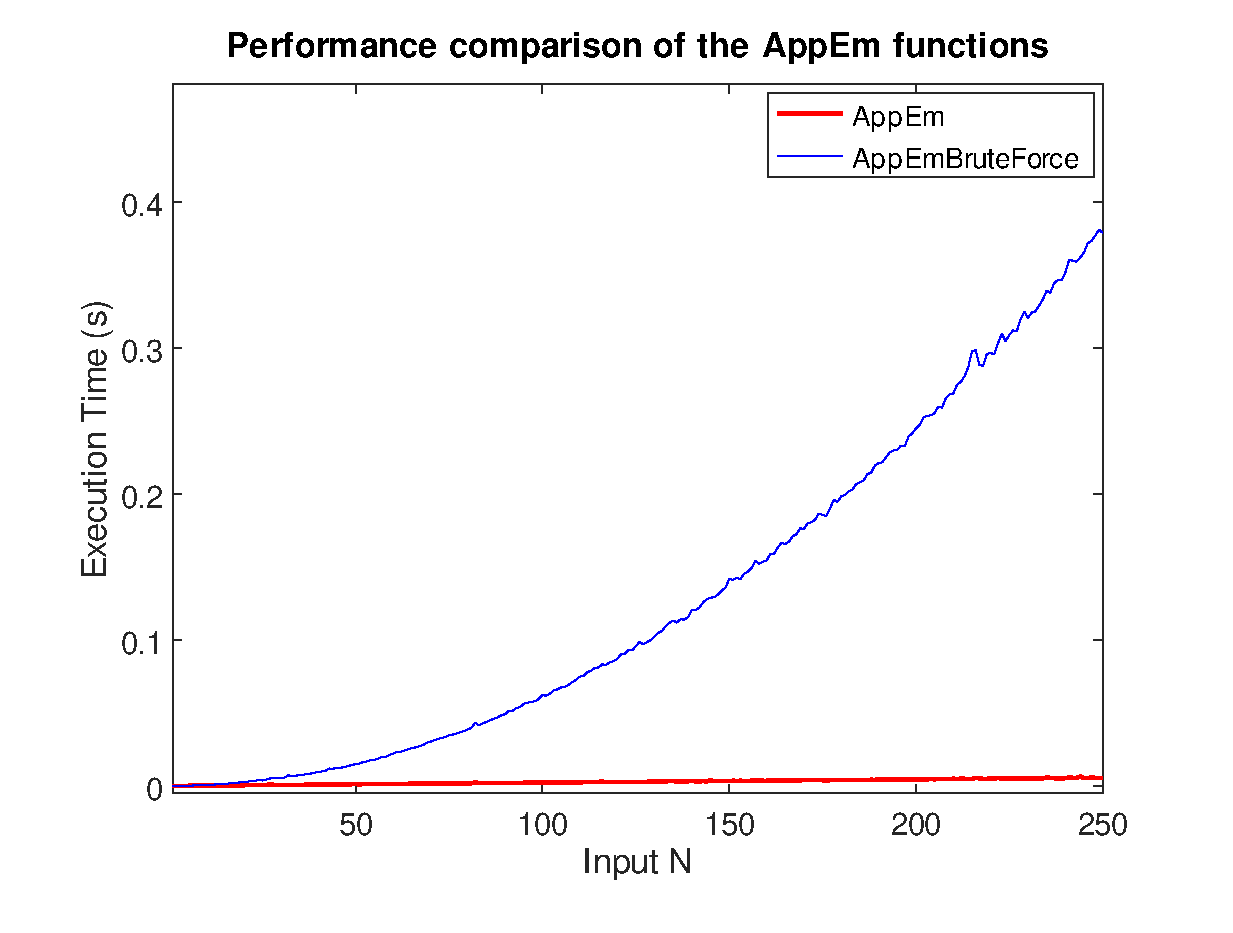
\includegraphics[scale=0.6]{bruteforce_vs_better.eps}

   \caption{A performance comparison between the brute force algorithm and the optimized version}
      \label{fig:emnaive_vs_better}
\end{figure}
\end{center}

\subsection{A specific example}

Let's consider the case that $N = 2019$. 

  \lstinputlisting[label={appem_test_code}, caption={A test of both implementations for N = 2019}] {../part1/part1.m}
  
Running the code in Listing \ref{appem_test_code} gives the following output

\begin{verbatim}
>> test_2019
p =  228
q =  395
Elapsed time is 0.0487769 seconds.
p =  228
q =  395
Elapsed time is 18.8509 seconds.
\end{verbatim}}

We see the output from both approaches are in agreement, and that the optimizations result in an almost 400 times speed up.

\begin{thebibliography}{9}
\bibitem{eulerconst}
Weisstein, Eric W. "Euler-Mascheroni Constant." From MathWorld--A Wolfram Web Resource. http://mathworld.wolfram.com/Euler-MascheroniConstant.html
Referenced: 22-02-2019


\end{thebibliography}

\end{document}
